\documentclass[conference]{IEEEtran}
\IEEEoverridecommandlockouts

\usepackage{cite}
\usepackage{amsmath,amssymb,amsfonts}
\usepackage{graphicx}
\usepackage{textcomp}
\usepackage{xcolor}
\usepackage{pgfgantt}
\usepackage{booktabs}
\usepackage{enumitem}
\usepackage{array}
\usepackage{hyperref}

\graphicspath{{img/}}
\def\BibTeX{{\rm B\kern-.05em{\sc i\kern-.025em b}\kern-.08em
    T\kern-.1667em\lower.7ex\hbox{E}\kern-.125emX}}

\begin{document}

\title{K PLUS Adaptive Goal Allocation for First Jobbers\\
{\footnotesize History-Aware Payday Cash Allocation under Uncertain Cash Flows}}

\author{\IEEEauthorblockN{Anonymous Submission}
\IEEEauthorblockA{\textit{K PLUS First Jobber Hackathon --- Track 2: Data Science \& Intelligence}}
}

\maketitle

\begin{abstract}
First Jobbers must divide a limited monthly surplus between immediate liquidity, an emergency buffer, and a short-term financial goal. A fixed saving rule ignores the fact that future essential expenses and income volatility differ across users. We formulate this decision as a six-cycle finite-horizon Markov decision process with hard allocation feasibility and an evaluated shortfall-risk constraint. The proposed K PLUS experience recommends an allocation at the payday moment while leaving the final decision with the user. The study compares a transparent fixed rule, known-model Dynamic Programming (DP), Bayesian adaptive DP, pooled Reinforcement Learning (RL), and a small recurrent Meta-RL policy. The recurrent policy receives no task label and updates its context from observed salary, expense, and reward history. All methods use the same simulator, action grid, reward, and matched evaluation paths. The primary research question is whether history-based Meta-RL improves held-out cash-flow adaptation enough to justify its complexity over Bayesian DP. The work is an auditable Track 2 experiment rather than a production banking integration or a claim about real customer outcomes.
\end{abstract}

\begin{IEEEkeywords}
First Jobber, sequential decision-making, Dynamic Programming, Bayesian adaptation, Meta-Reinforcement Learning, liquidity risk, financial goal allocation
\end{IEEEkeywords}

\section{Executive Summary: One-Page Pitch}

\subsection{Problem Statement}
First Jobbers often receive a regular salary but have little margin for unexpected expenses. At each payday they must decide how much surplus to keep liquid, place in an emergency buffer, or allocate to a personal goal. The decision changes the cash available in later cycles. A fixed percentage rule is unable to account for a user's changing shortfall risk. The supplied references support buffer-versus-consumption trade-offs and sequential goal allocation, but do not establish the prevalence of this problem among K PLUS customers. That prevalence remains a validation hypothesis.

\subsection{Proposed Solution}
K PLUS Adaptive Goal Allocation is an optional payday recommendation. It estimates near-term cash-flow uncertainty from observed history and recommends a feasible pair $(e_t,q_t)$: an emergency-buffer allocation and a goal allocation. The remaining surplus stays liquid. The explanation exposes the trade-off, for example, how allocating more to the goal changes the chance of an essential-expense shortfall. The prototype evaluates the policy in a controlled simulator; it does not move or lock real funds.

\subsection{Target Users}
The initial segment is salaried K PLUS users aged 22--30 with a small liquid buffer and one short-term savings goal. Users receive a decision that accounts for future uncertainty and preserves control over the final transfer. K PLUS gains a testable form of personalized financial decision support that can be evaluated before any production integration. Retention, deposits, debt reduction, and customer impact are not claimed by this proposal.

\subsection{Value Proposition}
\textbf{For First Jobbers:} The recommendation makes the reserve-versus-goal trade-off visible at the payday moment. It can reduce avoidable essential-expense shortfalls in the simulator while preserving progress toward a user-selected goal. Users can inspect a counterfactual allocation and accept, edit, or reject the suggestion.

\textbf{For K PLUS/KBank:} The concept creates a small, testable decision-support experience around an existing salary and savings context. It provides an auditable way to evaluate personalization and trust before requesting production data or automatic transfers. Business outcomes such as retention, deposits, or credit risk are hypotheses for later validation, not results of this proposal.

\subsection{Track Perspective}
Track 2 is demonstrated through an explicit MDP, a DP oracle, posterior-based adaptation, and a controlled Meta-RL comparison. Meta-RL is a falsifiable candidate method. If Bayesian DP performs equally well, the simpler method is the appropriate result.

\section{Introduction}\label{sec:introduction}

Financial goal management is sequential: an allocation today changes the liquidity and attainable goals available at the next payday. A First Jobber may have stable salary income but still face a low-probability expense shock. Allocating too much to a goal can create a shortfall; allocating too little can make a goal unreachable. Buffer behavior under uncertain income is a classic dynamic consumption-saving problem~\cite{deaton}, while goals-based wealth management uses dynamic optimization to trade off competing future goals~\cite{dasdp}.

Recent work applies Meta-RL to goals-based wealth management (GBWM) by pre-training policies over many multi-year investment problems~\cite{dasmeta}. That work chooses investment portfolios and whether to fulfil scheduled goals, and reports zero-shot inference for new problem parameters. Our proposal studies a different, smaller decision: how to allocate payday surplus between an emergency buffer, one accumulating goal, and liquid cash. The user task type is hidden at evaluation time and must be inferred from observed cash-flow history. There is no portfolio optimization or real banking data.

The proposal makes three deliberate choices. First, DP is implemented before model-free learning because the horizon and state grid are small. Second, Bayesian DP is a strong adaptation baseline because it explicitly represents uncertainty about the hidden cash-flow dynamics. Third, the recurrent Meta-RL policy is included only to test whether learned history compression provides value beyond that baseline. This ordering prevents algorithmic complexity from replacing a clear problem definition.

\subsection{Research Questions}
\begin{enumerate}[noitemsep,topsep=2pt]
    \item Does known-model DP improve the goal-attainment and liquidity-risk frontier over a tuned fixed allocation rule?
    \item When the cash-flow type is unknown, does Bayesian DP retain an advantage over a pooled policy using the same observations?
    \item Does a recurrent Meta-RL policy adapt on held-out task dynamics well enough to outperform Bayesian DP, or is Meta-RL unnecessary for this problem?
\end{enumerate}

The contributions are an auditable small MDP, a matched comparison of sequential policies, and an explicit complexity gate for Meta-RL. The work does not propose a new Meta-RL algorithm or claim that a simulated improvement transfers automatically to K PLUS customers.

\section{Project Scope}\label{sec:project_scope}

\subsection{In-Scope Elements}
\begin{itemize}[noitemsep,topsep=2pt]
    \item \textbf{Decision:} one allocation at each of six monthly payday cycles among liquid cash, one emergency buffer, and one optional goal.
    \item \textbf{Environment:} salary arrival, a fixed essential obligation, variable expenses, occasional shocks, and configurable reserve withdrawal friction.
    \item \textbf{Methods:} fixed-split, reserve-first and goal-first rules; known-model DP; Bayesian DP; pooled tabular RL; and a recurrent Meta-RL prototype.
    \item \textbf{Evaluation:} held-out cash-flow paths, held-out task dynamics, mild distribution shifts, paired bootstrap intervals, and policy ablations.
    \item \textbf{K PLUS experience:} an optional payday explanation and allocation suggestion that leaves execution to the user.
\end{itemize}

\subsection{Out-of-Scope Elements}
The MVP excludes investment portfolios and market returns, multi-year multi-goal wealth management, fraud detection, credit underwriting, debt origination, cross-bank aggregation, automatic money movement, customer identity data, regulated financial advice, and a production-scale mobile or backend system. These exclusions keep the experiment focused on one intervention and make the result reproducible without K PLUS infrastructure.

\subsection{Assumptions and Constraints}
Salary and essential expenses are observed at cycle boundaries. The simulator uses declared synthetic distributions rather than Thai population estimates. Goal and reserve weights are explicit experiment or user inputs; Meta-RL does not infer a user's moral preferences. The reserve can be drawn only after liquid cash is exhausted, with withdrawal friction exposed as a sensitivity parameter. Results are conditional on these assumptions.

\subsection{Booklet Alignment}
\begin{itemize}[noitemsep,topsep=1pt,leftmargin=*]
    \item \textbf{Problem Statement:} First Jobbers must allocate limited surplus while future shortfall risk is uncertain.
    \item \textbf{Proposed Solution:} A history-aware payday allocation recommendation with an explanation of the liquidity trade-off.
    \item \textbf{Target Users:} Salaried 22--30-year-old users with a small buffer and one short-term goal; this is a validation hypothesis.
    \item \textbf{Value Proposition:} Easier, more risk-aware allocation for users and an auditable Track 2 personalization experiment for K PLUS.
    \item \textbf{Track Perspective:} MDP formulation, DP benchmark, Bayesian belief update, and a held-out Meta-RL test.
\end{itemize}

\section{Project Requirements}\label{sec:project_requirements}

\subsection{Functional Requirements}
\begin{itemize}[noitemsep,topsep=2pt]
    \item \textbf{FR1:} The simulator shall generate a seeded six-cycle trajectory with salary and expense outcomes for a declared hidden task type.
    \item \textbf{FR2:} Each policy shall select only feasible discrete allocations satisfying $e_t+q_t\leq m_t$.
    \item \textbf{FR3:} DP shall enumerate finite-support transitions and expose action values for inspection.
    \item \textbf{FR4:} Bayesian DP shall update a posterior over task types from observed salary and expense outcomes.
    \item \textbf{FR5:} Pooled RL and recurrent Meta-RL shall train on the same task distribution without receiving the task label at evaluation.
    \item \textbf{FR6:} Evaluation shall run all policies on identical pre-generated paths and report reward, goal attainment, reserve attainment, shortfall probability, shortfall amount, and terminal liquidity.
    \item \textbf{FR7:} The experiment shall include grid refinement, task-type ablations, history ablations, and at least one distribution shift.
\end{itemize}

\subsection{Non-Functional Requirements}
\begin{itemize}[noitemsep,topsep=2pt]
    \item \textbf{Reproducibility:} all random seeds, simulator parameters, action grids, and evaluation paths are recorded.
    \item \textbf{Auditability:} DP transitions and policy actions can be inspected for a given state.
    \item \textbf{Fairness of comparison:} methods share the same reward, feasibility rules, horizon, and observation budget.
    \item \textbf{Scope control:} the core experiment runs locally with NumPy and does not require APIs, GPUs, or live customer data.
    \item \textbf{Safety of communication:} outputs are recommendations for a simulator study and are not presented as guaranteed financial advice.
\end{itemize}

\subsection{Data Requirements and Strategy}
The MVP requires synthetic initial balances, a fixed-obligation schedule, task-specific salary and expense distributions, one goal target and deadline, reward weights, and shared evaluation seeds. A later study could calibrate distributions using anonymized aggregate statistics, but raw transaction histories and customer identifiers are not required. The simulator and experiment outputs are versioned with the code so that a claimed improvement can be reproduced.

\section{Solution Design}\label{sec:solution_design}

\subsection{Decision Environment}
At decision time $t$, the state is
\[
s_t=(t,w_t,r_t,g_t,d_t,y_t,f_t),
\]
where $w_t$ is liquid cash, $r_t$ is the reserve, $g_t$ is goal progress, $d_t$ is time to deadline, and $y_t,f_t$ are current salary and fixed obligation. The available surplus is $m_t=[w_t+y_t-f_t]_+$. The discrete action is $a_t=(e_t,q_t)$ with $e_t,q_t\geq0$ and $e_t+q_t\leq m_t$. Remaining surplus stays liquid.

After the action, a variable expense $X_t$ is drawn from the hidden task type $\theta$. Liquid cash pays first; the reserve covers the remainder; any uncovered amount is a shortfall. The next state is
\[
w_{t+1}=[m_t-e_t-q_t-X_t]_+,\quad
r_{t+1}=r_t+e_t-v_t,\quad
g_{t+1}=g_t+q_t.
\]
The step reward combines covered essentials, shortfall cost, and useful reserve growth. Terminal reward records goal attainment, reserve attainment, and remaining liquid cash:
\[
J(\pi;\theta)=\mathbb{E}\left[\sum_{t=0}^{T-1}\rho_t+\rho_T\right].
\]
The probability of any shortfall is reported as a risk metric; its limit is tested by penalty and sensitivity sweeps rather than treated as an unsupported production guarantee.

\subsection{Policy Comparison}
Known-model DP computes the Bellman recursion
\[
V_t(s)=\max_{a\in A(s)}\mathbb{E}_{s'\sim P_\theta}[\rho(s,a,s')+V_{t+1}(s')].
\]
When $\theta$ is unknown, Bayesian DP maintains a belief $b_t(\theta)$ and uses the posterior-predictive transition. Pooled Q-learning tests model-free control without history inference. The recurrent Meta-RL policy is trained over task types and updates a hidden context from observed state, previous outcome, and reward:
\[
z_t=\operatorname{RNN}_\psi(z_{t-1},o_t),\qquad
a_t\sim\pi_\phi(a_t\mid s_t,z_t).
\]
The task label is never passed to the recurrent policy. This is the proposed user-adaptation mechanism. The implementation is intentionally a small policy-gradient prototype; a recurrent PPO implementation is an optional extension, not a requirement for claiming a result.

\begin{figure}[htbp]
\centerline{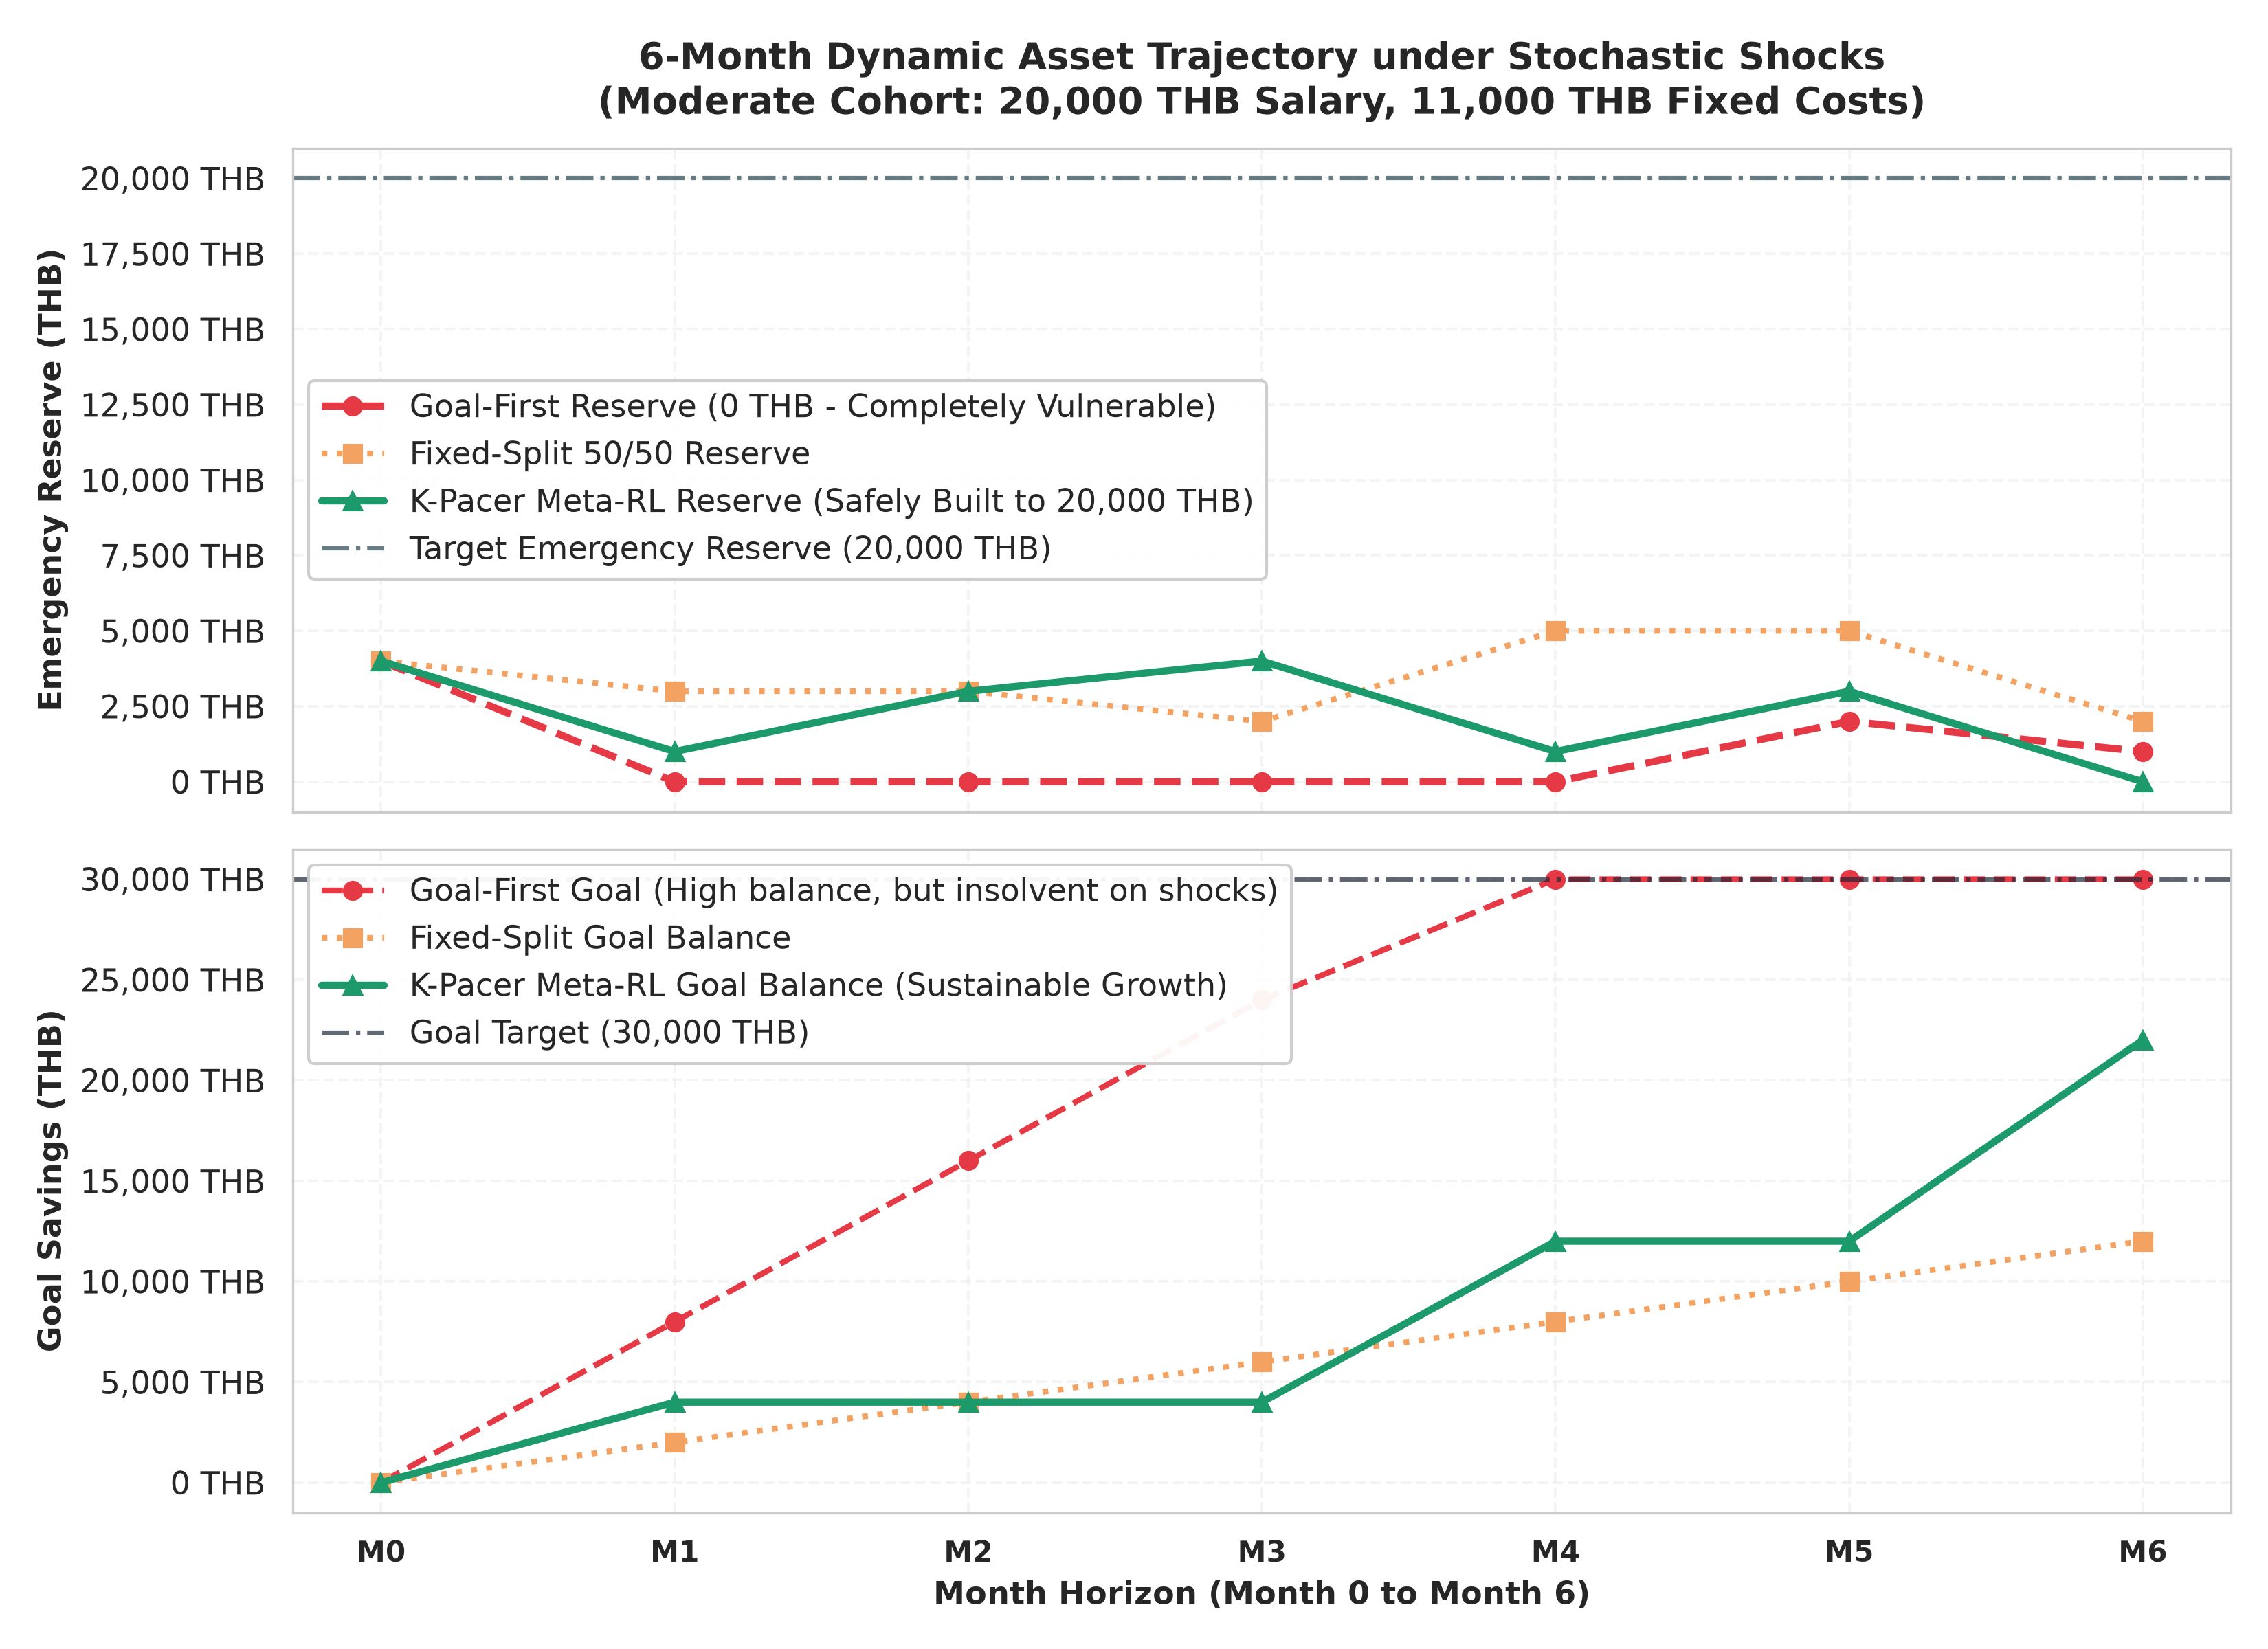
\includegraphics[width=\columnwidth]{trajectory_simulation.png}}
\caption{Example matched cash-flow trajectories from the controlled simulator.}
\label{fig:trajectory}
\end{figure}

\subsection{User Experience and Explainability}
At payday, K PLUS can present one recommended allocation and a counterfactual: how the suggested amount changes goal progress, reserve coverage, and simulated shortfall risk. The user can edit or reject the recommendation. The prototype does not transfer funds. This intervention is deliberately small enough to validate as a single decision moment.

\subsection{Track 2 Contribution}
The technical contribution is the decision-making experiment: a common finite MDP, a model-based optimum, uncertainty-aware adaptation, and a falsifiable test of recurrent context. Adding Meta-RL without a held-out adaptation gain does not count as success. If Bayesian DP matches the recurrent policy, Bayesian DP is retained as the more interpretable Track 2 method.

\begin{figure}[htbp]
\centerline{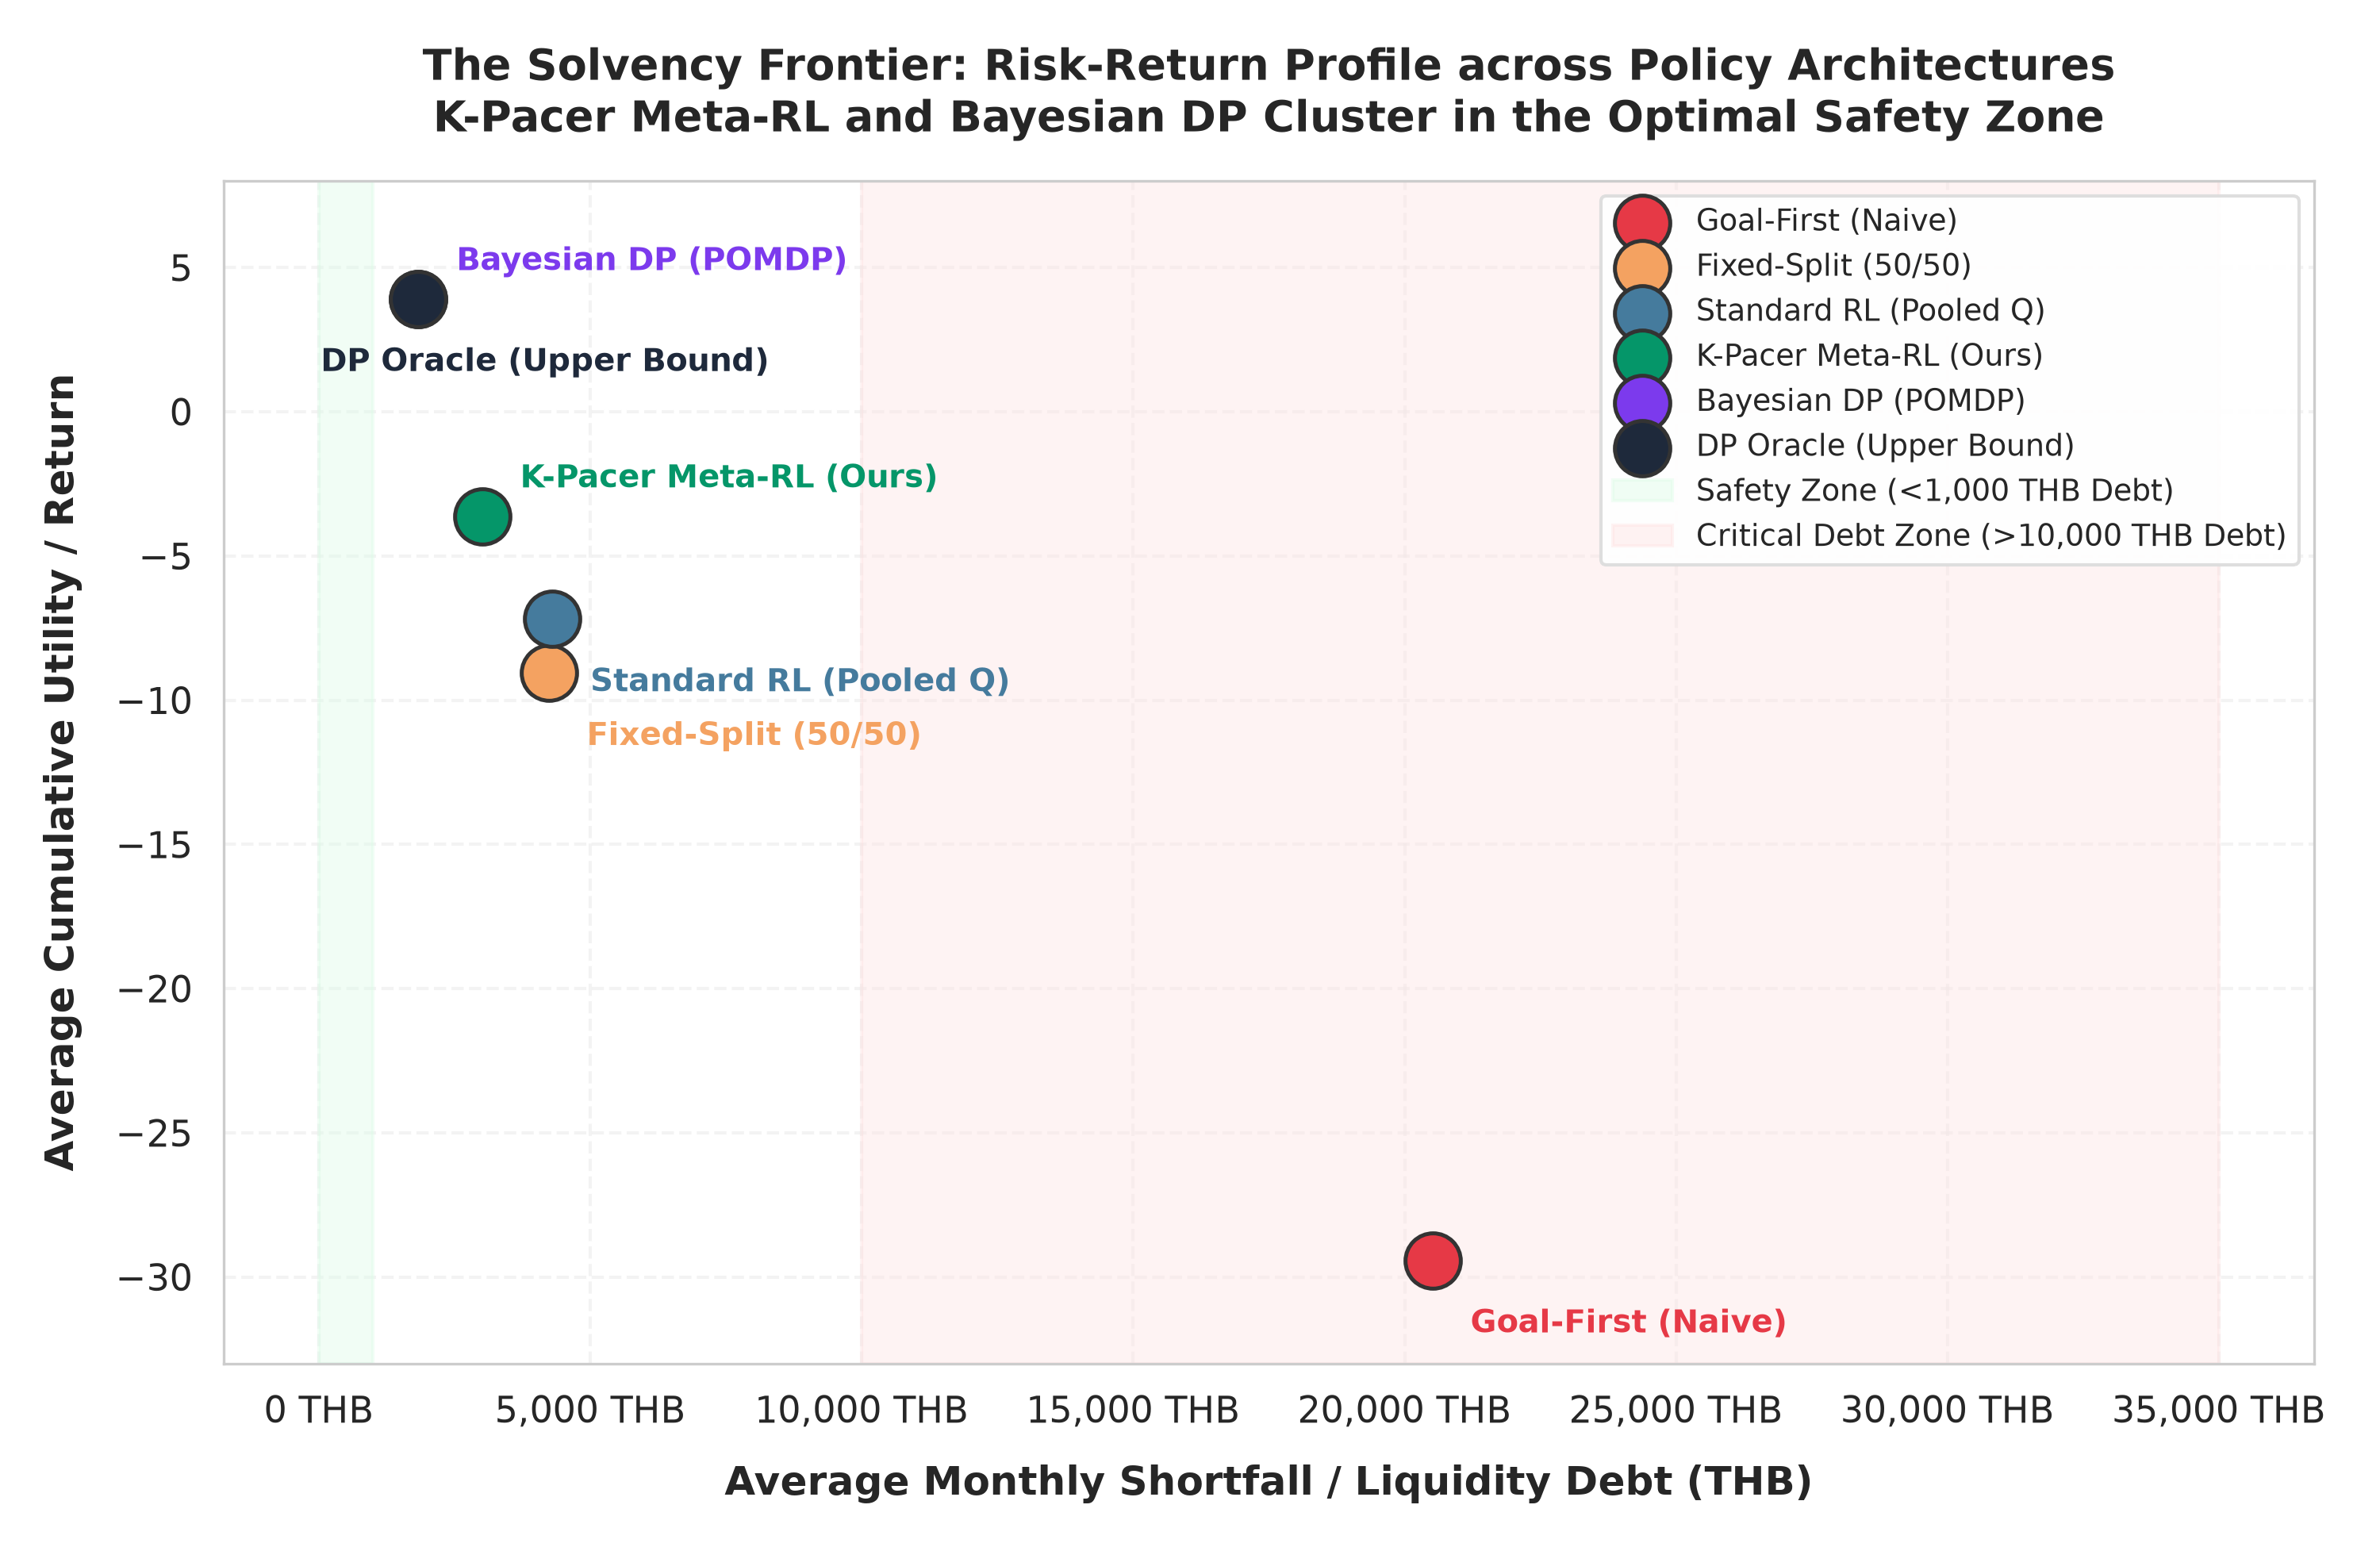
\includegraphics[width=\columnwidth]{safety_frontier.png}}
\caption{Example reward versus shortfall-risk frontier used for policy comparison.}
\label{fig:frontier}
\end{figure}

\section{Project Plan}\label{sec:project_plan}

\subsection{Implementation Phases}
\begin{itemize}[noitemsep,topsep=2pt]
    \item \textbf{Phase 1 --- Environment (Days 1--3):} implement seeded transitions, feasibility checks, reward accounting, and hand-verified two-cycle cases.
    \item \textbf{Phase 2 --- Model-Based Baselines (Days 4--6):} add fixed rules, exact DP, grid refinement, and Bayesian posterior updates.
    \item \textbf{Phase 3 --- Learned Policies (Days 7--10):} train pooled Q-learning and the recurrent Meta-RL prototype with task-randomized episodes.
    \item \textbf{Phase 4 --- Evaluation (Days 11--13):} generate matched held-out paths, run task shifts and ablations, and compute paired bootstrap intervals.
    \item \textbf{Phase 5 --- Pitch and Review (Days 14--15):} produce the policy comparison, explainability example, scope statement, and final Track 2 proposal.
\end{itemize}

\subsection{Timeline}
\begin{figure}[htbp]
\centerline{\resizebox{\columnwidth}{!}{
\begin{ganttchart}[hgrid,vgrid,x unit=0.43cm,y unit chart=0.38cm,
    bar height=0.55,group height=0.45,bar label font=\scriptsize,
    group label font=\scriptsize]{1}{15}
    \gantttitle{Days}{15}\\
    \gantttitlelist{1,...,15}{1}\\
    \ganttgroup{Environment}{1}{3}\\
    \ganttbar{Transitions and tests}{1}{3}\\
    \ganttgroup{DP baselines}{4}{6}\\
    \ganttbar{DP and Bayesian DP}{4}{6}\\
    \ganttgroup{RL methods}{7}{10}\\
    \ganttbar{Pooled Q and Meta-RL}{7}{10}\\
    \ganttgroup{Evaluation}{11}{13}\\
    \ganttbar{Held-out paths and ablations}{11}{13}\\
    \ganttgroup{Pitch}{14}{15}\\
    \ganttbar{Analysis and proposal}{14}{15}
\end{ganttchart}}}
\caption{Fifteen-day implementation and evaluation plan.}
\label{fig:gantt}
\end{figure}

\subsection{Deliverables}
The deliverables are the seeded simulator, unit tests, policy implementations, reproducible evaluation artifacts, a short policy explanation, and this proposal. The experiment can be demonstrated without a frontend or a banking API.

\section{Feasibility Analysis}\label{sec:feasibility_analysis}

\subsection{Technical Feasibility}
The environment has a finite horizon, discrete action grid, finite-support transitions, and three declared task types. These properties make exact DP feasible on a laptop and provide an oracle for learned policies. The current implementation uses Python and NumPy only. The main engineering risks are state-grid growth, unstable policy-gradient updates, and simulator misspecification; all can be exposed by grid checks, multiple seeds, and distribution-shift tests.

\subsection{Experimental Protocol}
Policies are trained only on declared training tasks. Evaluation uses unseen random seeds, interpolation task types, and at least one increased-shock condition. Every policy receives the same pre-generated salary and expense paths. Results are reported by task type, not only as a population average. Primary metrics are expected total reward, goal attainment, reserve attainment, any-shortfall probability, conditional shortfall amount, terminal liquidity, adaptation gain after the first two cycles, and compute cost.

\subsection{Risk Assessment}
\begin{table}[htbp]
\caption{Research and product risks with mitigations.}
\centering\scriptsize
\begin{tabular}{p{1.55cm}p{2.1cm}p{3.15cm}}
\toprule
\textbf{Risk} & \textbf{Why it matters} & \textbf{Mitigation}\\
\midrule
Simulator bias & A policy may optimize artificial cash flows. & Publish parameters; vary shocks, weights, and reserve friction; report conditional claims.\\
Fake adaptation & A recurrent network may use capacity without identifying task dynamics. & Compare Bayesian DP, pooled RL, no-history ablations, and task-type oracle.\\
Reward hacking & Reserve preservation may starve liquid spending. & Report all component metrics and inspect action traces.\\
Grid artifacts & Coarse DP may create a false optimum. & Refine balance and action grids; report stability.\\
Preference sensitivity & Weights determine the goal/liquidity trade-off. & Treat weights as explicit inputs and run sensitivity analysis.\\
Product overclaim & Simulation does not prove user impact. & Keep the feature optional; exclude real-money movement and production claims.\\
\bottomrule
\end{tabular}
\label{tab:risks}
\end{table}

\subsection{Business and Ethical Feasibility}
The proposed intervention fits an existing payday or goal-planning moment and can be prototyped without privileged banking access. A user retains control over the transfer decision. The system should explain uncertainty and show counterfactuals rather than present a guaranteed recommendation. Real customer deployment would require product research, consent, privacy controls, suitability review, and calibration with aggregate data; none is claimed here.

\section{Conclusion}\label{sec:conclusion}

K PLUS Adaptive Goal Allocation reduces a broad financial-assistant idea to one decision: how to divide payday surplus between liquidity, an emergency buffer, and one short-term goal when future cash flow is uncertain. The proposed study follows a research progression from transparent rules to DP, Bayesian adaptation, pooled RL, and recurrent Meta-RL. This produces a meaningful Track 2 result even if the simplest method wins. A Meta-RL claim is accepted only when the recurrent policy improves held-out adaptation over Bayesian DP under matched observations and remains stable under distribution shift. The project is therefore small enough for a student team to implement and deep enough to test sequential decision-making rather than prediction alone.

\section{Relationship to the Supplied Research}\label{sec:relationship}

The proposal is inspired by Das et al.'s Meta-RL formulation for goals-based wealth management~\cite{dasmeta}, but the decision problem is intentionally different. The supplied paper selects investment portfolios and fulfils scheduled goals over multi-year wealth paths. This project allocates monthly surplus to an emergency reserve, one accumulating goal, and liquid cash. The paper reports zero-shot generalization from problem parameters; this project tests whether a recurrent policy can infer a hidden cash-flow type from short interaction history. The comparison is a small, falsifiable application study rather than a reproduction or a new Meta-RL algorithm.

\input{sections/references}

\end{document}
